\chapter{Resultados}
\label{cap4}


\FloatBarrier

\paragraph{} A partir dos modelos criados na Seção \ref{sub:super_models} e dos parâmetros refinados na Seção \ref{sub:est_simulation}, é possível prosseguir com as simulações finais, que compartilham das seguintes configurações:

\begin{itemize}
    \item 71 \textit{tickers} (Tabela \ref{tab:5})
    \item Período de simulação: 01/04/2020 a 31/12/2021
    \item Capital: R\$ 100000,00
    \item Volume mínimo de ações por negociação: 1
    \item Risco de entrada por operação: 0,29
    \item Período máximo de dias por operação: 45
\end{itemize}

\paragraph{} Observa-se que o período de simulação é posterior ao utilizado para refinamento dos parâmetros de simulação (01/01/2019 a 31/12/2020).

\paragraph{} A Tabela \ref{tab:395} mostra 4 perfis de simulação diferentes, cada um motivado por uma questão diferente, são elas: (1) o máximo local na região de baixo RCC da Figura \ref{fig:550}; (2) o máximo local da região de alto RCC, também da Figura \ref{fig:550}; (3) a simulação de maior índice de Sharpe da Figura \ref{fig:153} e pertencente à curva \begin{math} RCC \times K = 1,8 \end{math}; e (4) a simulação de menor perda de operações na Figura \ref{fig:155}, pertencente à curva \begin{math} RCC \times K = 0,1 \end{math}. Também são apresentados os respectivos resultados.


% Estratégia 1: ID=250
% Estratégia 2: ID=251
% Estratégia 3: ID=252
% Estratégia 4: ID=253
\begin{table}[!htb]
    \begin{center}
        \resizebox{\textwidth}{!}{
        \begin{tabular}{ l|c|c|c|c|c }
            Parâmetro & Estratégia 1 & Estratégia 2 & Estratégia 3 & Estratégia 4 & \textit{Baseline} \\
            \hline
            RCC                                 & 0,11\%        & 6,10\%        & 0,00288\%     & 0,1\%         & - \\
            K                                   & -             & -             & 62500         & 100           & - \\
            \hline
            Rendimento Final                    & 15,90\%       & -17,45\%      & -2,34\%       & 33,25\%       & 68,07\% \\
            Volatilidade                        & 17,18\%       & 53,77\%       & 43,00\%       & 31,81\%       & 34,84\% \\
            Índice de Sharpe                    & 0,45          & -0,14         & 0,02          & 0,67          & 1,15 \\
            Índice de Sortino                   & 0,67          & -0,15         & 0,02          & 0,99          & 1,71 \\
            Cor. Spearman (\textit{Baseline})   & 0,96          & 0,39          & 0,18          & 0,90          & - \\
            Cor. Spearman (Ibovespa)            & 0,98          & 0,48          & 0,26          & 0,93          & - \\
            Uso Máximo de Capital               & 71,75\%       & 100\%         & 100\%         & 99,98\%       & 100\% \\
            Uso Médio de Capital                & 52,63\%       & 99,36\%       & 97,85\%       & 92,29\%       & 100\% \\
            Média de Cap. por Op.               & R\$1112,69    & R\$2038,49    & R\$2042,67    & R\$2145,08    & - \\
            Desvio P. de Cap. por Op.           & R\$434,26     & R\$11673,90   & R\$6601,82    & R\$2247,61    & - \\
            % Máximo de Op. Ativas                &  &  &  &  & 71 \\
            % Média de Op. Ativas                 &  &  &  &  & 71 \\
            % Desvio Padrão de Op. Ativas         &  &  &  &  & - \\
            Operações Totais                    & 1663          & 418           & 1171          & 1659          & 71 \\
            Operações de Sucesso                & 371 (22,3\%)  & 92 (22,0\%)   & 262 (22,4\%)  & 370 (22,3\%)  & - \\
            Operações de Falha                  & 1060 (63,7\%) & 250 (59,8\%)  & 753 (64,3\%)  & 1057 (63,7\%) & - \\
            Operações de \textit{Timeout}       & 164 (9,9\%)   & 66 (15,8\%)   & 104 (8,9\%)   & 164 (9,9\%)   & - \\
            Operações Incompletas               & 68 (4,1\%)    & 10 (2,4\%)    & 52 (4,4\%)    & 68 (4,1\%)    & - \\
        \end{tabular}}
        \caption{Resultados finais}
        \label{tab:395}
    \end{center}
\end{table}

\paragraph{} As Figuras \ref{fig:731}, \ref{fig:732}, \ref{fig:733} e \ref{fig:734} apresentam os rendimentos ao longo do tempo das 4 estratégias supracitadas.

\begin{figure}[!htb]
    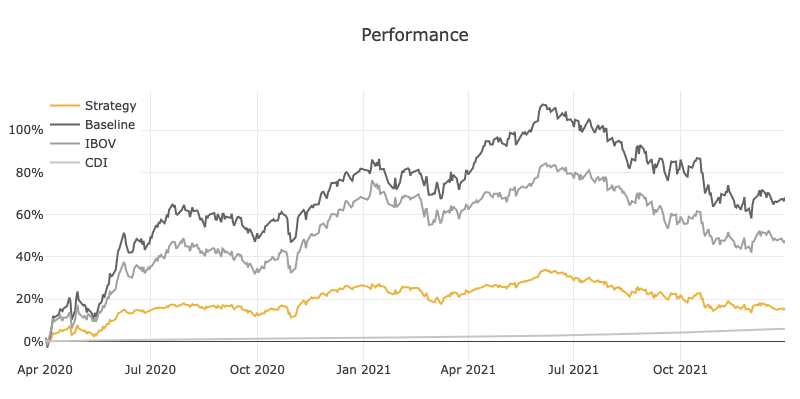
\includegraphics[scale=0.50]{yield_strategy_1.png}
    \centering
    \caption{Rendimento da Estratégia 1}
    \label{fig:731}
\end{figure}

\begin{figure}[!htb]
    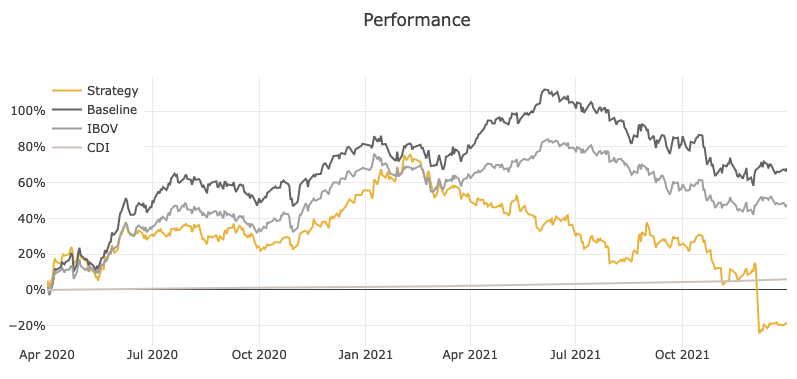
\includegraphics[scale=0.50]{yield_strategy_2.png}
    \centering
    \caption{Rendimento da Estratégia 2}
    \label{fig:732}
\end{figure}

\begin{figure}[!htb]
    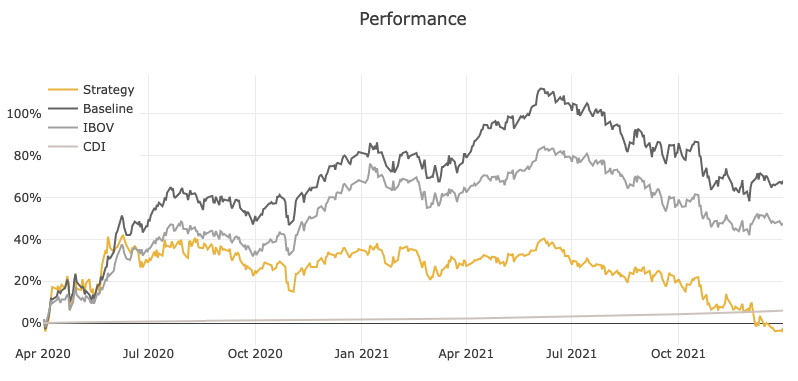
\includegraphics[scale=0.50]{yield_strategy_3.png}
    \centering
    \caption{Rendimento da Estratégia 3}
    \label{fig:733}
\end{figure}

\begin{figure}[!htb]
    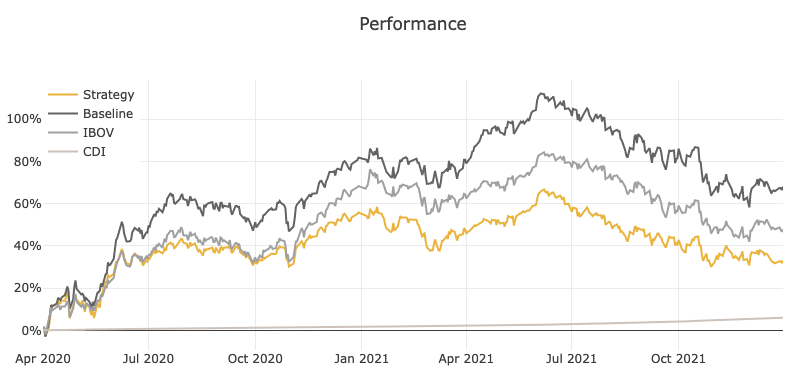
\includegraphics[scale=0.50]{yield_strategy_4.png}
    \centering
    \caption{Rendimento da Estratégia 4}
    \label{fig:734}
\end{figure}

\FloatBarrier

\paragraph{} Começando a análise pelos pontos em comum entre as estratégias, percebe-se que todas obtiveram o rendimento final, o índice de Sharpe e o índice de Sortino significativamente menor que o \textit{baseline}. Além disso, ficaram por baixo no gráfico de rendimento em quase todo o intervalo de simulação. A taxa de sucesso, de falha, de \textit{timeout} e de incompletude das operações se mantiveram praticamente constantes. Apenas a Estratégia 2 que apresentou um ruído maior, pois esta foi a que mais forçou o uso de capital ao máximo, o que conforme visto na Seção \ref{sub:risk_man}, traz mais instabilidade.

\paragraph{} É possível ver que a ordem de progressão do rendimento e dos índices de Sharpe e Sortino seguem o seguinte padrão ascendente: Estratégia 2, Estratégia 3, Estratégia 1 e Estratégia 4.

\paragraph{} A Estratégia 2 mostra que a escolha do RCC do segundo pico da Figura \ref{fig:550} certamente não foi uma boa escolha, pois seus indicadores de performance são os piores dentre as outras três estratégias. Tal resultado não é uma surpresa porque já foi verificado que a disputa por capital em uma região de altíssimo RCC ou K traz um efeito aleatório que ofusca a qualidade de atuação dos modelos, pois muitas operações deixam de existir para que outras monopolizem quase todo o capital da carteira. Verifica-se também o baixo número de operações realizadas em decorrência desse efeito (418), o que serve mais como um indicativo do nível de saturação ocorrido do que como um aspecto atrativo a um potencial investidor. Para saber o número total de operações perdidas devido à saturação de capital, basta uma comparação com o número de operações da Estratégia 1 (1663), já que a mesma possui um uso médio de capital de 52,63\%.

\paragraph{} O baixo rendimento e índice de Sharpe da Estratégia 3 em comparação às Estratégias 1 e 4 questiona o critério de escolha de um alto índice de Sharpe nas curvas apresentadas pela Figura \ref{fig:153}. Nota-se aqui também o alto uso médio de capital de 97,85\%, o que indica saturação. Esse efeito é significativamente menor que a Estratégia 2, pois nesta região assintótica da curva (rever Figura \ref{fig:550}), uma pequena diferença no uso médio de capital impacta bastante no desvio padrão do capital por operação, que por sinal cai quase pela metade entre ambas as estratégias.

\paragraph{} A Estratégia 1 possui cerca de 50\% de capital ocioso, o que não a impede de ser melhor que as Estratégias 2 e 3 sob o ponto de vista da performance e do índice de Sharpe. Tal resultado está relacionado ao enfraquecimento da influência dos modelos devido ao efeito aleatório decorrente da saturação de capital, o que não ficou evidente durante a análise da Figura \ref{fig:550}. Para reforçar, vale a menção de que as duas estratégias com maior rendimento e índice de Sharpe, as estratégias 1 e 4, são as que estão mais longe da saturação de capital. A Estratégia 1, dentre as quatro apresentadas, é a que tem menor volatilidade e isso contribui bastante para seu índice de Sharpe de 0,45. Esta também é a única estratégia que apresenta o desvio padrão de capital por operação menor que a média do mesmo. Isso revela uma melhor distribuição de capital entre todos os ativos da carteira.

\paragraph{} A análise sob a ótica das correlações de Spearman requer um pouco de cautela. Uma correlação muito próxima de 1 entre uma estratégia e sua referência pode indicar uma dependência muito alta, a ponto de atrapalhar na obtenção de ganhos acima da própria referência. Por outro lado, é importante analisar também as tendências de alta e de baixa do mercado, uma vez que não é desejável uma correlação alta com uma referência que só apresenta quedas, muito pelo contrário. Em suma, como regra geral, não se deseja uma correlação muito alta, pois é justamente nos espaços não correlacionados que uma estratégia tem abertura para se opor a uma tendência de mercado prejudicial a si mesma. Todavia, muita oposição pode indicar ineficiência.

\paragraph{} Portanto, verifica-se que a Estratégia 4, de maior rendimento e índice de Sharpe, possui uma correlação de Spearman com o \textit{baseline} um pouco menor que a Estratégia 1 (0,90 e 0,96, respectivamente). Já as estratégias 2 e 3 apresentaram as menores correlações (0,39 e 0,18, respectivamente).

\paragraph{} Em resumo, um investidor mais preocupado com a volatilidade poderia escolher a estratégia 1, já um outro investidor que priorize os ganhos ao custo de uma maior volatidade poderia escolher a Estratégia 4.
